\documentclass[]{article}
\usepackage{amsmath}
\usepackage{graphicx}
\usepackage{amssymb}
\newcommand{\reals}{\mathbb{R}}
\newcommand{\prox}{\textnormal{\textbf{prox}}}
\DeclareMathOperator*{\argmin}{arg\,min}
\DeclareMathOperator*{\argmax}{arg\,max}
\usepackage[margin=1in]{geometry}
\usepackage{parskip}

\usepackage{algorithm}
\usepackage[noend]{algpseudocode}

\begin{document}


\title{Technical Report: Autoencoder Kernel PCA}
\author{Jeremy Cohen, Elad Hazan, Tengyu Ma}
\date{\today}
\maketitle

\section{Introduction}
Dimensionality reduction is a widely-studied problem in data analysis and machine learning, with applications to compression, de-noising, and classification.
Given a sample of $n$ data points $\{\mathbf{x}_i\}_{i=1}^n \subset \reals^d$ drawn from some distribution $\mathcal{D}$, the goal is to learn an ``encoder'' $f: \reals^d \to \reals^k$ which preserves ``informative'' structure while discarding noise.
What makes for informative structure?
A number of popular dimensionality reduction techniques can be motivated by what might be termed the ``autoencoder principle'': an encoder $f$ learns informative structure in the data if there exists a decoder $g: \reals^k \to \reals^d$ which can accurately reverse the encoding to ``reconstruct'' the original data, so that $g(f(\mathbf{x})) \approx \mathbf{x}$ for all $\mathbf{x} \sim \mathcal{D}$.

Principal component analysis (PCA) is a linear dimensionality reduction technique which finds the $k$-dimensional subspace ``closest to'' the data.
From an autoencoding perspective, PCA finds the linear encoder $f(\mathbf{x}) = \mathbf{A} \mathbf{x}$ that minimizes the error in reconstructing the data points from their encodings.
On the one hand, PCA is simple to implement and computationally efficient: the basis vectors for this subspace are simply the eigenvectors of the empirical covariance matrix, and these can be computed via the singular value decomposition of the data matrix.
On the other hand, the underlying assumption that the data lie near a low-dimensional linear subspace is quite restrictive.

Kernel PCA \cite{scholkopf1997} uses some nonlinear mapping $\phi: \reals^d \to \mathcal{F}$ to transform the data points into a higher-dimensional ``feature space'' $\mathcal{F}$, and then performs PCA on the transformed data points $\phi(\mathbf{x}_1) \hdots \phi(\mathbf{x}_n)$.
For example, with a degree-$\ell$ polynomial kernel, the feature space is $\mathcal{F} = \reals^{d^\ell}$ and the feature map $\phi(\mathbf{x}) = \mathbf{x}^{\otimes \ell} $ takes the product of every group of $\ell$ dimensions. 
 The so-called ``kernel trick'' conveniently allows us to do PCA \textit{implicitly} in $\mathcal{F}$ without ever actually computing any $\phi(\mathbf{x}_i)$, so the resource requirements of the algorithm do not depend on $\text{dim}(\mathcal{F})$, which can even be infinite.
Kernel PCA can find non-linear structure in the data, but the catch is that it doesn't optimize an autoencoding objective.
Rather than try to reconstruct the \textit{original} data points $\mathbf{x}$ from their encoding $f(\phi(\mathbf{x}))$, kernel PCA tries to reconstruct the \textit{feature-mapped} data points $\phi(\mathbf{x})$ from their encodings $f(\phi(\mathbf{x}))$.
As a result, kernel PCA learns an encoder that retains information maximally informative of $\phi(\mathbf{x})$, whereas PCA learns an encoder that retains information maximally informative of $\mathbf{x}$ itself.
  

In this technical report, we present ``autoencoding kernel PCA'' (AKPCA), a cousin of PCA and kernel PCA which combines the best of both worlds: like kernel PCA, it can learn non-linear structure, but like PCA, its autoencoding objective tries to reconstruct the \textit{original data points} from a lower-dimensional encoding.

The objective function of autoencoding kernel PCA is almost identical to that of kernel PCA with a degree 2 polynomial kernel, except that it penalizes deviations from $\phi(\mathbf{x}_i) = \mathbf{x}^{\otimes 2}$ in the spectral norm rather than in the Frobenius norm.
This simple modification leads autoencoding kernel PCA to do a better job than kernel PCA in reconstructing the data points, but at the sacrifice of computational tractability: whereas kernel PCA can be solved exactly with an eigendecomposition, autoencoding kernel PCA is a challenging non-convex optimization problem that we can only tackle with heuristics like stochastic gradient descent.
Moreover, the time and space complexity of autoencoding kernel PCA is $O(k d^{2})$, which precludes its use in settings where the dimension $d$ is large.
For this reason, we also propose a ``data-span'' variant in which we restrict the decision variable to lie within the span of the data points mapped into feature space.
This hack brings the space complexity to $O(kn)$ and the time complexity to $O(nd)$, and is therefore feasible in settings where the dimension $d$ is large, but the number of data points $n$ is comparatively small.

We compare autoencoding kernel PCA (and its data-span variant) to PCA and kernel PCA on a reconstruction task, a denoising task and a classification task.
On the MNIST handwritten digits dataset, we find that AKPCA performs considerably better than the alternatives at reconstruction and denoising (at least when the noise level is small to moderate), while its performance on the classification task is mixed.
Unfortunately, AKPCA fails outperform the alternatives on any task on either the CIFAR-10 object recognition dataset or the Labeled Faces in the Wild face dataset.

We begin this technical report with a review of PCA and kernel PCA.
Then we introduce autoencoding kernel PCA and its data-span variant.
Finally, we report results of experiments on MNIST.

\section{Principal Components Analysis}

Principal component analysis (PCA), the simplest linear dimensionality reduction algorithm, finds a subspace that lies ``close'' to the data.
More specifically, given a set of data points $\mathbf{x}_1 \hdots \mathbf{x}_n \subset \reals^d$ stacked into the rows of a data matrix $\mathbf{X} \in \reals^{n\times d}$, PCA finds a $k$-dimensional linear subspace which minimizes the sum of the squared distances between the original data points and their projections onto the subspace.

To formulate PCA, let $\mathbf{a}_1 \hdots \mathbf{a}_k \subset \reals^d$ be an orthonormal basis for the optimal subspace, and let $\mathbf{A} = \begin{bmatrix} \mathbf{a}_1 & \hdots & \mathbf{a}_k \end{bmatrix}^T$.
Since the $\{\mathbf{a}_j\}_{j=1}^k$ are orthogonal, the projection $\Pi_{\mathbf{A}}(\mathbf{x})$ of any point $\mathbf{x} \in \reals^d$ onto the subspace they span is:
$$ \Pi_{\mathbf{A}}(\mathbf{x}) = \sum_{j=1}^k (\mathbf{a}_j ^T \mathbf{x}) \, \mathbf{a}_j = \mathbf{A}^T \mathbf{A} \mathbf{x}$$
So, to find the orthonormal vectors $\mathbf{a}_1 \hdots \mathbf{a}_k$ which minimize the sum of squared distances between $\mathbf{x}_i$ and $\Pi_{\mathbf{A}}(\mathbf{x}_i)$, we solve:
\begin{align}
\label{pca-opt}
\hat{\mathbf{A}} = \argmin_{\mathbf{A} \in \reals^{k \times d}} \; \sum_{i=1}^n \| \mathbf{x}_i - \mathbf{A}^T \mathbf{A} \mathbf{x}_i  \|_2^2 \quad \text{subject to} \quad \mathbf{A} \mathbf{A}^T = \mathbf{I}
\end{align}
It turns out that the solution to (\ref{pca-opt}) is to set $\mathbf{a}_1 \hdots \mathbf{a}_k$ to the $k$ eigenvectors of the empirical covariance matrix $\mathbf{X}^T \mathbf{X}$ with the largest eigenvalues, or equivalently, the $k$ right singular vectors of the data matrix $\mathbf{X}$.

Therefore, to perform PCA, one need only compute the singular value decomposition of $\mathbf{X}$ and set $\mathbf{A}$ to the $k$ leading right singular vectors.
Then the encoder is $f(\mathbf{x}) = \mathbf{A} \mathbf{x}$ and the decoder is $g(\mathbf{y}) = \mathbf{A}^T \mathbf{y}$.

\subsection{Centering}
PCA is often performed on centered data (i.e. where the mean of each dimension, over all data points, is zero).
The steps to perform PCA on centered data are:
\begin{enumerate}
\item
Compute the mean $\bar{\mathbf{x}} = \frac{1}{n} \sum_{i=1}^n \mathbf{x}_i$
\item
Compute the SVD of the centered data matrix,
$$ \tilde{\mathbf{X}} = \begin{bmatrix} \mathbf{x}_1 - \bar{\mathbf{x}} \\ \vdots \\ \mathbf{x}_n - \bar{\mathbf{x}} \end{bmatrix} $$
and let $\mathbf{A}$ be the matrix whose rows are the $k$ leading right singular vectors.
\item
The encoder is $f(\mathbf{x}) = \mathbf{A}(\mathbf{x} - \bar{\mathbf{x}})$ and the decoder is $g(\mathbf{y}) = \mathbf{A}^T \mathbf{y} + \bar{\mathbf{x}}$.
\end{enumerate}


%PROOF
%
%We can rewrite the difference as:
%$$ \| \mathbf{x} - \mathbf{A}^T \mathbf{A} \mathbf{x} \|^2_2 =  \sum_{j=1}^d (\mathbf{a}_j^T \mathbf{x}) \, \mathbf{a}_j  -  \sum_{j=1}^k (\mathbf{a}^T_j \mathbf{x}) \, \mathbf{a}_j =  \sum_{j=k+1}^d (\mathbf{a}^T_j \mathbf{x}) \, \mathbf{a}_j $$
%Taking the 2-norm, the cross-terms disappear because the $\{ \mathbf{a}_j \}$ are orthogonal,
%$$ \| \mathbf{x} - \mathbf{A}^T \mathbf{A} \mathbf{x} \|^2_2 =  \sum_{j=k+1}^d (\mathbf{a}_j^T \mathbf{x})^2 =  \sum_{j=k+1}^d \mathbf{a}_j^T \mathbf{x} \mathbf{x}^T \mathbf{a}_j$$
%Over all points in the dataset,
%$$ \argmin_{\mathbf{a}_{k+1} \, \hdots \, \mathbf{a}_d} \; \sum_{j=k+1}^d \mathbf{a}_j^T \left( \sum_{i=1}^n \mathbf{x}_i \mathbf{x}_i^T \right) \mathbf{a}_j \quad \text{such that} \quad \mathbf{a}_{k+1} \, \hdots \, \mathbf{a}_d \; \text{are orthonormal} $$
%The solution is where $\mathbf{a}_{k+1} \, \hdots \, \mathbf{a}_d$ are the $(d - k)$ eigenvectors of  $\sum_{i=1}^n \mathbf{x}_i \mathbf{x}_i^T $ with the smallest eigenvalues --- it follows that $\mathbf{a}_1 \hdots \, \mathbf{a}_k$ should be the $k$ eigenvectors with the \textit{largest} eigenvalues.
%
%The vectors $\mathbf{a}_1 \hdots \, \mathbf{a}_k \subseteq \reals^d$  are called the ``principal components'' of $\{\mathbf{x}_i\}_{i=1}^n$.

\section{Kernel PCA}

Kernel PCA \cite{scholkopf1997} is a dimensionality reduction algorithm which maps the data points to a higher-dimensional ``feature space'' using a non-linear mapping, and then performs PCA on the mapped data points. 

\subsection{Motivating Example}
Suppose that we observe data in $\reals^2$ from two different classes: red and blue.
The red data lies on the circle centered at the origin with radius $\frac{1}{2}$, while the blue data lies on the circle with radius $1$.

Notice that we cannot learn a linear classifier to distinguish red from blue points --- the two classes are not linearly separable.
Moreover, even if we use PCA to learn an encoding $\reals^2 \to \reals$, the classes are still not separated in the encoded data.

\begin{figure}[h]
\begin{center}
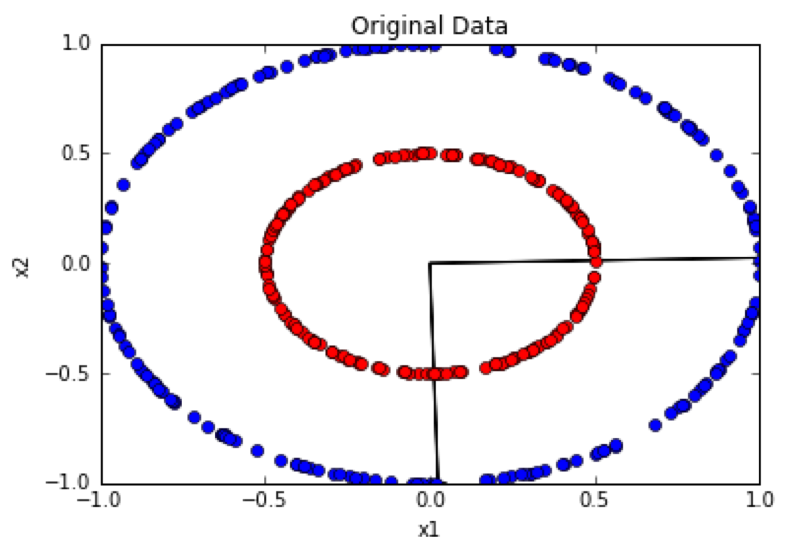
\includegraphics[scale=0.4]{figures/nonsep_data.png}
\quad \quad
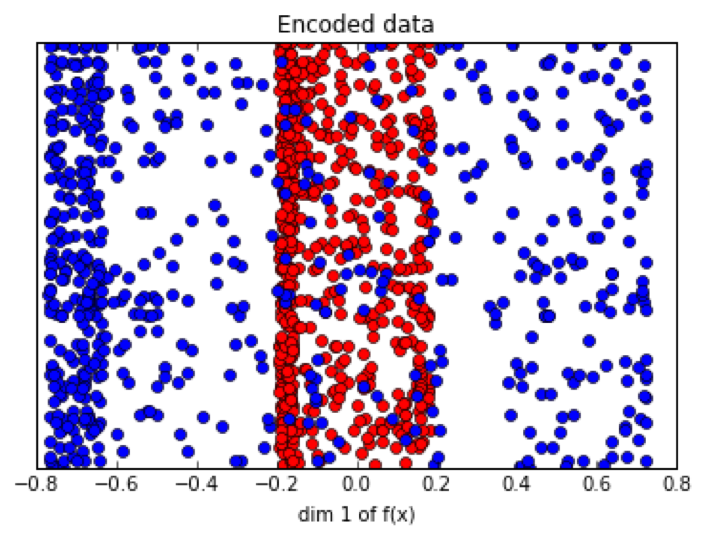
\includegraphics[scale=0.4]{figures/nonsep_data_pca.png}
\caption{Original data in $\reals^2$ (left) and the same data encoded into $\reals$ using PCA (right).}
\label{redblue}
\end{center}
\end{figure}

However, suppose that we map each data point to  degree-2 polynomial ``feature space'' with the map:
$$ \phi \left(\begin{bmatrix} x_1 \\ x_2 \end{bmatrix} \right) = \begin{bmatrix} x_1^2 \\ 2x_1 x_2 \\ x_2^2 \end{bmatrix} $$
In feature space, the red circle $x_1^2 + x_2^2 = \frac{1}{4}$ lies completely within the plane $\{a, b, c : a + c = \frac{1}{4} \}$, while the blue circle $x_1^2 + x_2^2 = 1$ lies within the parallel plane $\{a + c = 1 \}$; hence, the two classes are separated.
Sure enough, if we project the data onto the first principal component in feature space (the green arrow in figure \ref{redblue-2}, left), then we verify that the data are separated by class.

\begin{figure}[h]
\begin{center}
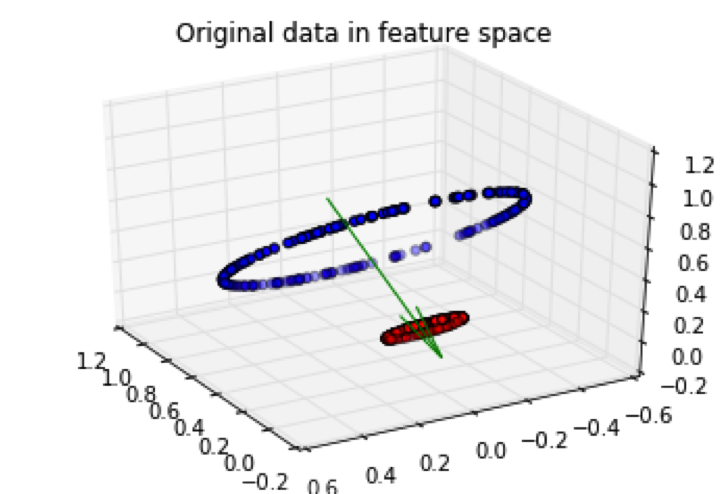
\includegraphics[scale=0.4]{figures/3d}
\quad \quad
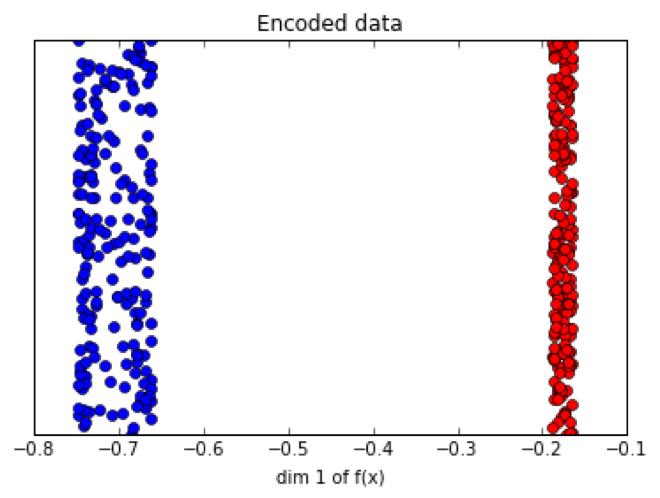
\includegraphics[scale=0.4]{figures/3d_encode}
\caption{Data from figure \ref{redblue} mapped in $\reals^3$ ``feature space'' using the degree-2 polynomial map (left), and the projection of this transformed data onto the first principal component (right). }
\label{redblue-2}
\end{center}
\end{figure}



\subsection{The Kernel Trick}

The naive way to perform PCA on data in feature space would be to explicitly map each data point into feature space, form the $n \times \text{dim}(\mathcal{F})$ matrix
$\boldsymbol{\Phi} = \begin{bmatrix} \phi(\mathbf{x}_1) & \hdots & \phi(\mathbf{x}_n) \end{bmatrix}^T$, and compute its top $k$ right singular vectors.

Unfortunately, this approach scales poorly with the dimension of $\mathcal{F}$: on a dataset with 1,000 images of size $100 \times 100$, this approach would require 
over 370 GB of memory just to form and store the transformed data matrix $\boldsymbol{\Phi}$!\footnote{as a matrix of 32-bit floating point numbers}

Fortunately, the so-called ``kernel trick'' is a shortcut that allows us to perform PCA in feature space without actually mapping the points into $\mathcal{F}$.
In fact, we will see that the runtime of kernel PCA does not depend at all on $\text{dim}(\mathcal{F})$.
The ``kernel trick'' is as follows: for certain feature maps $\phi: \reals^d \to \mathcal{F}$, one can compute the inner product $\phi(\mathbf{x})^T \phi(\mathbf{y})$ between two points in feature space without computing either $\phi(\mathbf{x})$ or $\phi(\mathbf{y})$.
Since PCA only accesses the data points through their pairwise inner products, we can do PCA in feature space without explicitly mapping the data points there.
The function $K(\mathbf{x}, \mathbf{y}) = \phi(\mathbf{x})^T \phi(\mathbf{y})$ is called the \textit{kernel} associated with the feature map $\phi$ \cite{scholkopf2002}.


For the degree-$\ell$ polynomial feature map $\phi(\mathbf{x}) = \mathbf{x}^{\otimes \ell}$, the corresponding kernel is \begin{align}\phi(\mathbf{x})^T \phi(\mathbf{y}) = (\mathbf{x}^T \mathbf{y})^\ell
\end{align}

%It turns out that many functions $K: \reals^d \times \reals^d \to \reals$ are equivalent to the inner product in some feature space.
%Specifically, $K$ is a valid kernel for some feature map $\phi$ if the \textit{kernel matrix} $\mathbf{K}$ defined for any data set $\mathbf{x}_1 \hdots \mathbf{x}_n$ with $K_{ij} = K(\mathbf{x}_i, \mathbf{x}_j)$, is a positive definite matrix for any $\mathbf{x}_1 \hdots \mathbf{x}_n$ 

We now show that the kernel trick allows us to solve kernel PCA via the eigendecomposition of an $n \times n$ matrix.

%The space complexity is kernel PCA is $O(n^2)$, to store the kernel matrix, while the time complexity is $O(n^2 d + n^2k )$, since the costliest operations are constructing the kernel matrix and computing its top $k$ eigenvectors.

\subsection{Derivation}

Let $\phi: \reals^d \to \mathcal{F}$ be a feature map with corresponding kernel $K: \reals^d \times \reals^d \to \reals$.

Let  $\boldsymbol{\Phi}$ be the matrix whose rows are the data points mapped into feature space:
$$\boldsymbol{\Phi} = \begin{bmatrix} \phi(\mathbf{x}_1) \\ \vdots \\ \phi(\mathbf{x}_n) \end{bmatrix}$$
To solve PCA in feature space, we need to find the $k$ leading eigenvectors of the covariance matrix of $\mathbf{\Phi}$,
\begin{align}
 \mathbf{C} = \frac{1}{n} \sum_{i=1}^n \phi(\mathbf{x}_i) \, \phi(\mathbf{x}_i)^T
\end{align}
Each such eigenvector/value pair ($\mathbf{v}$, $\lambda$) will satisfy the eigenvector equation 
\begin{align*}
\mathbf{C} \mathbf{v} = \lambda \mathbf{v}
\end{align*}
It follows that for any data point $\mathbf{x}_{\ell}$, an eigenvector/value pair $(\mathbf{v}, \lambda)$ must also satisfy
\begin{align}
\label{ev-equation}
\phi(\mathbf{x}_{\ell})^T \mathbf{C} \mathbf{v} = \lambda \, \phi(\mathbf{x}_\ell)^T \mathbf{v}
\end{align}
This gives us $n$ equations, one for each data point $\ell \in \{1 \hdots n\}$.

Now, since an eigenvector of $\mathbf{C}$ is by definition a vector $\mathbf{v}$ that satisfies $\sum_{i=1}^n \phi(\mathbf{x}_i) \phi(\mathbf{x}_i)^T \mathbf{v} = \lambda \mathbf{v}$, we know that any eigenvector of $\mathbf{C}$ is a linear combination of the data points in feature space:
\begin{align}
\label{linear-combo}
\mathbf{v} = \sum_{i=1}^n \alpha_i \, \phi(\mathbf{x}_i)
\end{align}
with $\alpha_i  = \frac{\phi(\mathbf{x}_i)^T \mathbf{v}}{\lambda}$.

Therefore, rather than solving for $\mathbf{v} \in \mathcal{F}$ directly, we may instead solve for the linear combination coefficients $\boldsymbol{\alpha} \in \reals^n$.

Plugging (\ref{linear-combo}) into (\ref{ev-equation}), we see that each $\boldsymbol{\alpha}$ must satisfy: 
\begin{align}
\phi(\mathbf{x}_{\ell})^T \mathbf{C} \left( \sum_{i=1}^n \alpha_i \, \phi(\mathbf{x}_i) \right) = \lambda \, \phi(\mathbf{x}_\ell)^T \sum_{i=1}^n \alpha_i \, \phi(\mathbf{x}_i)
\end{align}
Plugging in the definition of $\mathbf{C}$,
\begin{align}
\label{the-equation}
\phi(\mathbf{x}_{\ell})^T \left(  \frac{1}{n} \sum_{j=1}^n \phi(\mathbf{x}_j) \, \phi(\mathbf{x}_j)^T \right) \left( \sum_{i=1}^n \alpha_i \, \phi(\mathbf{x}_i) \right) = \lambda \, \phi(\mathbf{x}_\ell)^T \sum_{i=1}^n \alpha_i \, \phi(\mathbf{x}_i)
\end{align}
Rearranging both sides separately,
\begin{align}
\frac{1}{n} \sum_{i=1}^n \alpha_i \sum_{j=1}^n\phi(\mathbf{x}_{\ell})^T \phi(\mathbf{x}_j) \, \phi(\mathbf{x}_j)^T  \phi(\mathbf{x}_i)  = \lambda \, \sum_{i=1}^n \alpha_i \, \phi(\mathbf{x}_\ell)^T \phi(\mathbf{x}_i)
\end{align}
The inner products in feature space may be computed using the kernel function:
\begin{align}
\label{replace-with-kernel}
\frac{1}{n} \sum_{i=1}^n \alpha_i \sum_{j=1}^n k(\mathbf{x}_{\ell}, \mathbf{x}_j) \, k(\mathbf{x}_j, \mathbf{x}_i) = \lambda \, \sum_{i=1}^n \alpha_i \, k(\mathbf{x}_{\ell}, \mathbf{x}_i)
\end{align}
Which may be written using the kernel matrix $K_{ij} = k(\mathbf{x}_i, \mathbf{x}_j)$ as:
\begin{align*}
\frac{1}{n} \sum_{i=1}^n \alpha_i \langle \mathbf{K}_{\ell,:}, \mathbf{K}_{:,i} \rangle &= \lambda \langle \mathbf{K}_{\ell,:}, \boldsymbol{\alpha} \rangle \\
\frac{1}{n}  \langle \mathbf{K}_{\ell,:}, \mathbf{K} \boldsymbol{\alpha} \rangle &= 
\end{align*}
Since this relation must hold true for all $\ell \in \{1 \hdots n\}$, we may stack these $n$ equations on top of each other into the matrix equation:
\begin{align}
\label{kk}
\mathbf{K} \mathbf{K} \boldsymbol{\alpha} = n \lambda \mathbf{K} \boldsymbol{\alpha} 
\end{align}
Unless $\mathbf{K}$ has a zero eigenvalue, we may pre-multiply both sides by $\mathbf{K}^{-1}$ to obtain an eigenvalue problem:
\begin{align}
\label{eigenvalue-problem}
\mathbf{K} \boldsymbol{\alpha} = \nu \boldsymbol{\alpha} \quad \text{where} \quad \nu = n \lambda
\end{align}

\subsection{Normalization}

Finally, to ensure the uniqueness of the solution, we scale each principal component $\mathbf{v} \in \mathcal{F}$ to have unit norm.
It turns out that we can do this without ever computing $\mathbf{v}$ explicitly.
Let $\tilde{\boldsymbol{\alpha}}$ be a unit-norm eigenvector of $\mathbf{K}$ with eigenvalue $\nu$.
We seek a scaling $\boldsymbol{\alpha} \propto \tilde{\boldsymbol{\alpha}}$ such that $\| \mathbf{v} \| = 1$.

Since $\mathbf{v} = \sum_{i=1}^n \alpha_i  \, \phi(\mathbf{x}_i) = \Phi^T \boldsymbol{\alpha}$,
$$ \mathbf{v}^T \mathbf{v} = \boldsymbol{\alpha}^T \boldsymbol{\Phi} \boldsymbol{\Phi}^T \boldsymbol{\alpha} = \boldsymbol{\alpha}^T \mathbf{K} \boldsymbol{\alpha}  = \nu \, \boldsymbol{\alpha}^T\boldsymbol{\alpha} $$
where the last equality is because $\boldsymbol{\alpha}$ is an eigenvector of $\mathbf{K}$, c.f. (\ref{eigenvalue-problem}).
Therefore, to ensure that $\| \mathbf{v} \| = 1$, it suffices to have $\| \boldsymbol{\alpha}\| = \sqrt{\frac{1}{ \nu }}$.
We therefore take $\boldsymbol{\alpha} = \tilde{\boldsymbol{\alpha}} / \sqrt{\nu}$.

\subsection{Procedure}

In summary, to perform kernel PCA on data $\mathbf{X} \in \reals^{n \times d}$, we form the $n \times n$ kernel matrix $\mathbf{K}$, compute its $k$ leading eigenvectors, and divide each one by the square root of the corresponding eigenvalue.
Each resulting $\boldsymbol{\alpha}_j \in \reals^n$ are the coefficients of a kernel principal component expressed as a linear combination of the input data in feature space.

Having learned $\mathbf{A} = \begin{bmatrix} \boldsymbol{\alpha}_1 & \hdots & \boldsymbol{\alpha}_k \end{bmatrix}^T$, we can encode any data point $\mathbf{x}$ without ever computing $\phi(\mathbf{x})$.
The inner product of $\phi(\mathbf{x})$ with the $j$-th kernel principal component is 
\begin{align*}
\phi(\mathbf{x})^T \mathbf{v}_j &= \phi(\mathbf{x})^T  \left( \sum_{i=1}^n \alpha^j_i \, \phi(\mathbf{x}_i) \right) \\
&=  \sum_{i=1}^n \alpha^j_i \, k(\mathbf{x}, \mathbf{x}_i) \\
&= \mathbf{k}^T \boldsymbol{\alpha}^j \quad \text{where} \quad k_i = k(\mathbf{x}, \mathbf{x}_i)
\end{align*}
Therefore,
\begin{align}
f(\mathbf{x}) = \mathbf{A} \mathbf{k} \quad \text{where}  \quad k_i = k(\mathbf{x}, \mathbf{x}_i)
\end{align}

For the degree-$\ell$ polynomial kernel, it takes $O(n^2 d)$ time to compute the kernel matrix and $O(n^2k)$ time to compute its $k$ leading eigenvectors and eigenvalues.
Therefore, the overall runtime is $O(n^2 d)$, since when doing dimensionality reduction we have $k < d$.

\subsection{Centering}

Recall that PCA is often performed on centered data.
It turns out that there is a way to perform kernel PCA on data that is centered in feature space without ever explicitly mapping the data to feature space, much less computing the mean of the data there.
Let $\bar{\phi}(\mathbf{x})$ be a ``centered'' data point in feature space:
$$  \tilde{\phi}(\mathbf{x}) = \phi(\mathbf{x}) - \frac{1}{n} \sum_{j=1}^n \phi(\mathbf{x}_j) $$
and let $\tilde{\mathbf{K}}$ be the kernel matrix of the centered data, i.e. $\tilde{K}_{ij} = \tilde{\phi}(\mathbf{x}_i)^T \tilde{\phi}(\mathbf{x}_j)$
Simple algebra can show that the centered kernel matrix may be computed as:
$$\tilde{\mathbf{K}} =  \mathbf{K} - \mathbf{1}_n \mathbf{K}  - \mathbf{K} \mathbf{1}_n + \mathbf{1}_n \mathbf{K} \mathbf{1}_n \quad \text{where} \quad (\mathbf{1}_n)_{ij} = \frac{1}{n} $$
Having computed the centered kernel matrix, kernel PCA on centered data entails solving the eigenvector problem:
$$ \tilde{\mathbf{K}} \boldsymbol{\alpha} = \nu \boldsymbol{\alpha} $$

\subsection{Nystrom Approximation}

Both the space and time complexity of kernel PCA scale quadratically with the number of examples $n$.
For large datasets, we can instead use the Nystrom method \cite{williams2001} to solve kernel PCA approximately. 
A sample of $m$ data points is selected uniformly without replacement and the $k$ leading eigenvectors and eigenvalues $(\hat{\mathbf{v}}_1, \hat{\lambda}_1) \hdots (\hat{\mathbf{v}}_k, \hat{\lambda}_k)  $ of the resulting $m \times m$ kernel matrix are computed.
Then the eigenvectors and eigenvalues of the full kernel matrix are approximated as:
\begin{align}
\mathbf{v}_j &\approx \frac{\sqrt m}{n \, \hat{\lambda_j}} \mathbf{K} \hat{\mathbf{v}}_j \\
\lambda_j &\approx \frac{n}{m} \hat{\lambda}_j
\end{align}
where $\mathbf{K}$ is the $n \times m$ kernel matrix between the full data set and the sample. 

\section{Autoencoding Kernel PCA}

Kernel PCA is a richer model than PCA.
However, PCA's objective function has an easy autoencoding interpretation: compress $\mathbf{x}$ into a lower-dimensional representation and then try to reconstruct $\mathbf{x}$.
\begin{align*}
\argmin_{(f, g) \in \{f(\mathbf{x}) = \mathbf{A} \mathbf{x}, \, g(\mathbf{x}) = \mathbf{A}^T \mathbf{x} \}} \sum_{i=1}^n \|g(f(\mathbf{x}_i)) - \mathbf{x}_i \|^2_2 \tag{PCA objective}
\end{align*}
In contrast, kernel PCA's objective function compresses $\phi(\mathbf{x})$ into a lower-dimensional representation, and then tries to reconstruct $\phi(\mathbf{x})$.
\begin{align*}
\argmin_{(f, g) \in \{f(\mathbf{x}) = \mathbf{A} \mathbf{x}, \, g(\mathbf{x}) = \mathbf{A}^T \mathbf{x} \}} \sum_{i=1}^n \|g(f(\phi(\mathbf{x})_i)) - \phi(\mathbf{x}_i) \|^2_2 \tag{kernel PCA objective}
\end{align*}

We would expect PCA to learn an encoding function that is maximally informative of $\mathbf{x}$ itself, whereas we would expect kernel PCA to learn an encoding function that is maximally informative of  the degree-2 polynomial expansion $\phi(\mathbf{x})$.

In this section, we introduce ``autoencoding kernel PCA''  (AKPCA), a hybrid method which compresses $\phi(\mathbf{x})$ into a lower-dimensional representation, and then tries to reconstruct $\mathbf{x}$.

We will derive the AKPCA objective function from the same ``autoencoder'' principle as PCA: choose parameters of an encoder $f$ and a decoder $g$ so as to minimize the empirical reconstruction error,
$$ \sum_{i=1}^n \| g(f(\mathbf{x}_i)) - \mathbf{x}_i \|^2_2 $$

Our encoder will take the same form as in kernel PCA:
$$ f(\mathbf{x}) = \mathbf{A} \phi(\mathbf{x}) $$
parameterized by some matrix $\mathbf{A} \in \reals^{k \times d^2}$.

This raises the question: what is the natural decoder $g$ to decode kernel PCA encodings?
This is known as the ``pre-image problem'' in the kernel methods literature \cite{kwok2003, mika1999}, and it turns out that for the special case of a degree-2 polynomial kernel, the natural decoder involves solving an eigenvalue problem.

Given an encoding $f(\mathbf{x}) = \mathbf{A} \phi(\mathbf{x}) = \mathbf{y} \in \reals^k$, how can we recover some $\hat{\mathbf{x}}$ such that $f(\hat{\mathbf{x}}) = \mathbf{A} \phi(\hat{\mathbf{x}}) \approx \mathbf{y}$?
A natural way to start would be to premultiply $\mathbf{y}$ by $\mathbf{A}$, since the kernel PCA objective function guarantees that $\mathbf{A}^T \mathbf{y} = \mathbf{A}^T \mathbf{A} \phi(\mathbf{x})$ is close to $\phi(\mathbf{x})$.
But then how do we get from $\mathbf{A}^T \mathbf{y} \approx \phi(\mathbf{x})$ to $\hat{\mathbf{x}} \approx \mathbf{x}$?
We solve for the $\hat{\mathbf{x}}$ such that $\phi(\hat{\mathbf{x}})$ is closest to $\mathbf{z}: = \mathbf{A}^T \mathbf{y}$:
\begin{align*}
\hat{\mathbf{x}} &= \argmin_{\mathbf{x} \in \reals^d} \| \phi(\mathbf{x}) -  \mathbf{z}\|_2 \\
&=  \argmin_{\mathbf{x} \in \reals^d} \| \mathbf{x} \mathbf{x}^T -  \mathcal{M}(\mathbf{z})\|_F 
\end{align*}
By the Eckert-Young theorem, the best rank-1 approximation to $\mathcal{M}(\mathbf{y})$ is given by $\lambda_1 \mathbf{v}_1 \mathbf{v}_1^T$, where $(\mathbf{v}_1, \lambda_1)$ are the leading eigenvector and eigenvalue of $\mathcal{M}(\mathbf{y})$.
Therefore, the solution is $\hat{\mathbf{x}} = \sqrt{\lambda_1} \mathbf{v}_1$ if $\lambda_1  > 0$, or $\hat{\mathbf{x}} = \mathbf{0}$ if $\lambda_1 \le 0$.

Therfore, our decoder $g: \reals^{k} \to \reals^d$ should be defined as
$$ g(\mathbf{y}) = \max(\sqrt{\lambda_1}, 0) \mathbf{v}_1 \quad \text{where} \quad \mathbf{V} \boldsymbol{\Lambda} \mathbf{V}^T = \mathcal{M}(\mathbf{A}^T \mathbf{y})$$ 
Composing together the decoder and encoder, the natural autoencoding loss function is:
$$ \argmin_{\mathbf{A} \in \reals^{k \times d^2}} \sum_{i=1}^n \| \max(\sqrt\lambda_1, 0) \, \mathbf{v}_1(\mathcal{M}(\mathbf{A}^T \mathbf{A} \phi(\mathbf{x}))) - \mathbf{x}_i \|^2_2 $$

where we abuse notation by letting $\lambda_1$ and $\mathbf{v}_1$ denote the largest eigenpair of the matrix $\mathcal{M}(\mathbf{A}^T \mathbf{A} \phi(\mathbf{x}))$.

To make the model more flexible, we remove the restriction that the decoding matrix is the same as the encoding matrix, and optimize instead over two matrices $\mathbf{A}, \mathbf{B} \in \reals^{k \times d^2}$:
\begin{align}
\label{bad-objective}
 \argmin_{\mathbf{A}, \mathbf{B} \in \reals^{k \times d^2}} \sum_{i=1}^n \| \max(\sqrt\lambda_1, 0) \, \mathbf{v}_1(\mathcal{M}(\mathbf{B}^T \mathbf{A} \phi(\mathbf{x}))) - \mathbf{x}_i \|^2_2
\end{align}
It is not immediately clear how to optimize the objective function (\ref{bad-objective}) --- or even how to compute its gradient!
Therefore, we will instead optimize a surrogate objective function which comes out of the following inequality\footnote{We have not proved this inequality, but numerical simulations lead us to suspect that it is true.}: for any $\mathbf{x} \in \reals^d$ and $\mathbf{M} \in \reals^{d \times d}$,
\begin{align}
\label{the-inequality}
\| \max(\sqrt\lambda_1, 0) \, \mathbf{v}_1(\mathbf{M}) - \mathbf{x} \|^2_2 \le c \| \mathbf{M} - \mathbf{x} \mathbf{x}^T \|_2
\end{align}
for some small constant $c$, where $\| \cdot \|_2$ on the RHS of (\ref{the-inequality}) denotes the spectral norm of a matrix.

By employing inequality (\ref{the-inequality}) with $\mathbf{M} = \mathcal{M}(\mathbf{B}^T \mathbf{A} \phi(\mathbf{x}))$, we can see that the following objective function is an upper bound on (\ref{bad-objective}) to within a constant factor of $c$:
\begin{align}
\label{akpca-objective}
 \argmin_{\mathbf{A}, \mathbf{B} \in \reals^{k \times d^2}} \; \sum_{i=1}^n \| \mathcal{M}(\mathbf{B} \mathbf{A} \phi(\mathbf{x}_i) - \phi(\mathbf{x}_i)) \|_2
\end{align}
An alternative way to write the objective function (\ref{akpca-objective}) is:
\begin{align}
\label{akpca-objective-unraveled}
 \argmin_{\mathbf{A}, \mathbf{B} \in \reals^{k \times d^2}}  \; \sum_{i=1}^n \left \| \sum_{j=1}^k (\mathbf{x}_i^T \mathbf{A}_j \mathbf{x}_i) \mathbf{B}_j  - \mathbf{x}_i \mathbf{x}_i^T \right \|_2
\end{align}
where $\mathbf{A} = \begin{bmatrix} \text{vec}(\mathbf{A}_1) & \hdots & \text{vec}(\mathbf{A}_k) \end{bmatrix}^T$ and $\mathbf{B} = \begin{bmatrix} \text{vec}(\mathbf{B}_1) & \hdots & \text{vec}(\mathbf{B}_k)
\end{bmatrix}^T$.

The AKPCA objective function (\ref{akpca-objective-unraveled}) is \textit{almost} identical to the KPCA objective function (with a degree-2 polynomial kernel), but not quite: both methods try to choose $\{\mathbf{A}_j\}_{j=1}^k$ and $\{\mathbf{B}_j\}_{j=1}^k$ so as to approximate $\mathbf{x} \mathbf{x}^T$ with $\sum_k (\mathbf{x}^T \mathbf{A}_k \mathbf{x}) \mathbf{B}_k$.
The only difference is that AKPCA penalizes the residual  $\mathbf{x} \mathbf{x}^T - \sum_k (\mathbf{x}^T \mathbf{A}_k \mathbf{x}) \mathbf{B}_k$ in spectral norm, while KPCA does so in Frobenius norm.
Intuitively, reconstructing $\mathbf{x} \mathbf{x}^T$ to high accuracy in the spectral norm implies one can reconstruct $\mathbf{x}$ to high accuracy in $\ell_2$ norm.

\subsection{Optimization}

The AKPCA objective function (\ref{akpca-objective-unraveled}) is not convex, so we cannot hope to find a global optimizer.
Nevertheless, we found that running stochastic (sub)gradient descent or SVRG \cite{johnson2013} from a random starting point usually yielded a decent solution.

In what follows, we compute a subgradient of the AKPCA objective function
\begin{align*}
f(\mathbf{A}, \mathbf{B}) &= \left \| \sum_{j=1}^k \mathbf{x}^T \mathbf{A}_j \mathbf{x} \mathbf{B}_j  - \mathbf{x} \mathbf{x}^T \right \|_2 \\
&= \| \mathbf{M} \|_2 \quad \text{where} \quad \mathbf{M} =  \sum_{j=1}^k \mathbf{x}^T \mathbf{A}_j \mathbf{x} \mathbf{B}_j  - \mathbf{x} \mathbf{x}^T 
\end{align*}
The spectral norm is non-differentiable, so $f$ does not have a gradient.
Nevertheless, a subgradient of $f(\mathbf{M}) = \|\mathbf{M}\|_2$ is $\mathbf{u} \mathbf{v}^T$, where $\mathbf{u}$ and $\mathbf{v}$ are the leading left and right singular vectors of $\mathbf{M}$.

\textit{Derivative w.r.t. $\mathbf{A}_j$}

The derivative of $\mathbf{M}$ with respect to element $(r, s)$ of $\mathbf{A}_j$ is $x_r x_s \mathbf{B}_j$.
Therefore, by the chain rule,
$$ \frac{\partial f}{\partial A_{j, rs}} = \text{Tr}(\mathbf{v} \mathbf{u}^T x_r x_s \mathbf{B}_j) = x_r x_s \mathbf{u}^T \mathbf{B}_j \mathbf{v}$$
and
\begin{align}
\label{grad-a}
 \frac{\partial f}{\partial \mathbf{A}_j} = (\mathbf{u}^T \mathbf{B}_j \mathbf{v}) \mathbf{x} \mathbf{x}^T 
\end{align}

\textit{Derivative w.r.t. $\mathbf{B}_j$}

Similarly, the derivative of $\mathbf{M}$ with respect to element $(r, s)$ of $\mathbf{B}_j$ has  $\mathbf{x}^T \mathbf{A}_j \mathbf{x}$ at element $(r, s)$ and zeros everywhere else.
Therefore, by the chain rule, 
$$ \frac{\partial f}{\partial B_{j, rs}} = \mathbf{x}^T \mathbf{A}_j \mathbf{x} \, (\mathbf{u} \mathbf{v}^T)_{rs} $$
and
\begin{align}
\label{grad-b}
 \frac{\partial f}{\partial \mathbf{B}_j} = (\mathbf{x}^T \mathbf{A}_j \mathbf{x}) \, \mathbf{u} \mathbf{v}^T
\end{align}

The time and space complexity of AKPCA scale quadratically with the dimension $d$ of the data: it takes $O(k d^2)$ memory to store $\mathbf{A}$ and $\mathbf{B}$, and computing a stochastic subgradient estimator over a single data point takes $O(k d^2)$ time (see (\ref{grad-a}) and (\ref{grad-b})).
This quadratic dependence on $d$ renders AKPCA infeasible for high-dimensional data.
In the following section, we will present a ``hack'' that cuts the memory requirement to $O(kn)$ and the time complexity of computing a stochastic gradient estimator to $O(nd)$ --- at the cost of reducing the modeling power.


\section{Data-span Autoencoding KPCA}

Recall that even though kernel PCA was defined as an optimization problem in $\text{dim}(\mathcal{F})$ dimensions, it boiled down to an eigenvector problem in an $n \times n$ matrix because of the crucial fact that the eigenvectors of the covariance matrix of the data in feature space (i.e. the rows of $\mathbf{A})$ could be exactly represented as linear combinations of the data points in feature space. 

The same fact does not hold true for the AKPCA objective function: the rows of $\mathbf{A}$ and $\mathbf{B}$ at the optimal solution do not necessarily lie within the span of the data points in feature space.
Nevertheless, as a ``hack'' to render AKPCA tractable for datasets with large dimensionality $d$ but only small or moderate number of datapoints $n$, we may pretend as if this were true, and restrict each row of $\mathbf{A}$ to be a linear combination of the data points in feature space.
Rather than optimize over the $d^2$ entries of each row of $\mathbf{A}$ directly, we optimize over the $n$ coefficients of the linear combination.  
This ``data-span'' variant of AKPCA requires $O(kn)$ memory for storage and takes $O(nd)$ time to compute a stochastic gradient estimator.

\subsection{Derivation}

Let $h_{ij}$ be the contribution of data point $i$ to row $j$ of $\mathbf{A}$, so that:
$$ \mathbf{A}_{(j,:)} = \sum_{i=1}^n h_{ij} \, \mathbf{x}_i  $$
Define $g_{ij}$ in the same way for $\mathbf{B}$.

Let $\mathbf{h}_i = \begin{bmatrix} h_{i1} & \hdots & h_{ik} \end{bmatrix}^T$ and $\mathbf{g}_i = \begin{bmatrix} g_{i1} & \hdots & g_{ik} \end{bmatrix}^T$ be the contributions of data point $i$ to all rows of $\mathbf{A}$ and $\mathbf{B}$, respectively.

Let $\mathbf{H} = \begin{bmatrix} \mathbf{h}_1 \hdots \mathbf{h}_n \end{bmatrix} \in \reals^{k \times n}$ and $\mathbf{G} = \begin{bmatrix} \mathbf{g}_1 \hdots \mathbf{g}_n \end{bmatrix} \in \reals^{k \times n}$, so that the AKPCA parameters written as linear combinations of the data points in feature space are:
\begin{align}
\label{def-a}
\mathbf{A} &= \mathbf{H} \boldsymbol{\Phi} \\
\label{def-b}
\mathbf{B} &= \mathbf{G} \boldsymbol{\Phi} 
\end{align}
Under this new ``data-span'' parameterization, the term of the AKPCA objective function (\ref{akpca-objective}) for a data point $\mathbf{x}$ is:
\begin{align}
f(\mathbf{H}, \mathbf{G}) &= \left \| \mathcal{M}(\mathbf{B}^T \mathbf{A} \phi(\mathbf{x})) - \mathbf{x} \mathbf{x}^T \right \|_2  \nonumber \\
&= \| \mathcal{M}(\boldsymbol{\Phi}^T \mathbf{G}^T \mathbf{H} \boldsymbol{\Phi} \phi(\mathbf{x})) - \mathbf{x} \mathbf{x}^T \|_2 \tag{by (\ref{def-a}) and (\ref{def-b}) } \nonumber \\
&= \| \mathcal{M}(\boldsymbol{\Phi}^T \mathbf{G}^T \mathbf{H} \mathbf{k}) - \mathbf{x} \mathbf{x}^T \|_2 \nonumber  \tag{by the kernel trick} \\
\label{ds-objective}
&= \left \| \sum_{i=1}^n (\mathbf{G}^T \mathbf{H} \mathbf{k})_i \mathbf{x}_i \mathbf{x}_i^T  - \mathbf{x} \mathbf{x}^T \right \|_2  \\
&= \| \mathbf{M} \|_2 \quad \text{where} \quad \mathbf{M} = \sum_{i=1}^n z_i \mathbf{x}_i \mathbf{x}_i^T  - \mathbf{x} \mathbf{x}^T \quad \text{and} \quad \mathbf{z} = \mathbf{G}^T \mathbf{H} \mathbf{k}\nonumber
\end{align}
where $\mathbf{k} \in \reals^n$ denotes the vector obtained by applying the kernel function between $\mathbf{x}$ and each of $\mathbf{x}_1 \hdots \mathbf{x}_n$:
$$k_i =  \phi(\mathbf{x})^T \phi(\mathbf{x}_i) = (\mathbf{x}^T \mathbf{x}_i)^2$$

\subsection{Optimization}

Even though the data-span AKPCA objective function (\ref{ds-objective}) is not convex, we were able to attain a reasonable solution using stochastic gradient descent initialized from a random point.
In what follows, we compute a subgradient of (\ref{ds-objective}).

\textit{The derivative wrt z}:

Since $\mathbf{M}$ is symmetric, the derivative of $f$ w.r.t $\mathbf{M}$ is:
$$ \frac{\partial f}{\partial \mathbf{M}} = \mathbf{v} \mathbf{v}^T  $$
where $\mathbf{v}$ is the leading eigenvector of $\mathbf{M}$.

Moreover, from the definition of $\mathbf{M}$ it is clear that
$$\frac{\partial \mathbf{M}}{\partial z_i} = \mathbf{x}_i \mathbf{x}_i^T$$
Therefore, by the chain rule, 
\begin{align*}
 \frac{\partial f}{\partial z_i} &= \sum_{\text{elements of $\mathbf{M}$}} \frac{\partial f}{\partial \mathbf{M}} \frac{\partial \mathbf{M}}{\partial \mathbf{z}_i} \\
&= \text{Tr}((\mathbf{v} \mathbf{v}^T)^T (\mathbf{x}_i \mathbf{x}_i^T)) \\
&= (\mathbf{x}_i^T \mathbf{v})^2
\end{align*}
Equivalently, in vector form,
\begin{align}
\frac{\partial f}{\partial \mathbf{z}} &= (\mathbf{X} \mathbf{v})^2 \quad \text{where} \quad (\cdot)^2 \text{ is the element-wise square}
\end{align}

\textit{The derivative wrt $\mathbf{G}$}:

Since $\mathbf{z} = \mathbf{G}^T \mathbf{H} \mathbf{k}$, the $i$th element is given by  $z_i = \mathbf{g}_i^T\mathbf{H} \mathbf{k}$. 
Therefore, the derivative of $z_i$ w.r.t. the $i$th column of $\mathbf{G}$ is $\frac{\partial z_i}{\partial \mathbf{g}_i} = \mathbf{H} \mathbf{k}$.
Therefore, by the chain rule, the derivative of $f$ w.r.t. the $i$th column of $\mathbf{G}$ is:
$$ \frac{\partial f}{\partial \mathbf{g}_i} =   \frac{\partial f}{\partial z_i} \frac{\partial z_i}{\partial \mathbf{g}_i} = \frac{\partial f}{\partial z_i} \mathbf{H} \mathbf{k} $$
Equivalently, in matrix form,
\begin{align}
\frac{\partial f}{\partial \mathbf{G}}  = \mathbf{H} \mathbf{k} \frac{\partial f}{\partial \mathbf{z}}^T
\end{align}

\textit{The derivative wrt $\mathbf{H}$}:

Since $z_i = \mathbf{g}_i^T\mathbf{H} \mathbf{k}$, we have:
$$ \frac{\partial z_i}{\partial \mathbf{H}} = \mathbf{g}_i \mathbf{k}^T $$
Therefore, by the chain rule:
\begin{align}
\frac{\partial f}{\partial \mathbf{H}} &= \sum_{i=1}^n \frac{\partial f}{\partial z_i} \frac{\partial z_i}{\partial \mathbf{H}} \nonumber \\
&=  \sum_{i=1}^n \frac{\partial f}{\partial z_i} \left(  \mathbf{g}_i \mathbf{k}^T  \right) \nonumber \\
&= \left(  \sum_{i=1}^n \frac{\partial f}{\partial z_i} \mathbf{g}_i \right) \mathbf{k}^T \nonumber  \\
&= \mathbf{G} \frac{\partial f}{\partial \mathbf{z}} \mathbf{k}^T
\end{align}

\subsection{Efficiently computing the gradient}

It turns out that we can evaluate the DS-AKPCA objective function (\ref{ds-objective}) and compute its subgradient in $O(dn)$ time.
How could this be?
After all, forming $\mathbf{M}$ explicitly in memory would take $O(d^2)$ space and $O(n d^2)$ time!

The trick is to use the Lanczos algorithm to compute the leading eivenvector and eigenvalue of $\mathbf{M}$ without ever forming $\mathbf{M}$  explicitly.
The Lanczos algorithm only accesses $\mathbf{M}$ only through matrix-vector products $\mathbf{M} \mathbf{w}$; Lanczos requires $O(\frac{1}{\epsilon})$ of these matrix-vector multiplications to converge to an $\epsilon$-approximate solution.

The key matrix-vector multiplication takes the form:
$$ \mathbf{M} \mathbf{w} = \sum_{i=1}^n z_i \mathbf{x}_i \mathbf{x}_i^T \mathbf{w} - \mathbf{x} \mathbf{x}^T \mathbf{w} $$
which can be evaluated in $O(nd)$ time.

Of course, we first need to compute $\mathbf{z} =  \mathbf{G}^T \mathbf{H} \mathbf{k}$ in advance.
This takes $O(nd)$ time to compute $\mathbf{k}$, followed by $O(nk)$ time to compute $\mathbf{z}$.

Therefore, in total, computing the leading eigenvector and eigenvalue of $\mathbf{M}$ takes $O(nk + nd + \frac{nd}{\epsilon})$ time, where $\epsilon$ is the tolerance given to the Lanzcos algorithm.

Once we have the leading eigenvector, computing the subgradient of $f$ wrt $\mathbf{G}$ and $\mathbf{H}$ takes $O(n(d + k)$ time.

Since for dimensionality reduction the number of components $k$ is less than the dimensionality of the data $d$, the whole thing takes $O(nd(1 + \frac{1}{\epsilon}))$ time.

\section{Experiments}

We compared our two algorithms, AKPCA and DS-AKPCA, to PCA and kernel PCA (with a degree-2 polynomial kernel) on the MNIST handwritten digits dataset.
MNIST consists of 70,000 examples, each a 28x28 grayscale image of a digit with an integer label of 0 through 9.

We compared these four algorithms on several metrics: 
\begin{enumerate}
\item
Reconstruction error on the training set: $\sum_{i \in \text{train}} \| \mathbf{x}_i - g(f(\mathbf{x}_i)) \|_2^2$,
a measure of how large/flexible the model's hypothesis class is, and, for those algorithms that rely on non-convex optimization, a measure of how well the optimization succeeded.
\item
Reconstruction error on the held-out set:  $\sum_{i \not \in \text{train}} \| \mathbf{x}_i - g(f(\mathbf{x}_i)) \|_2^2$, a measure of how well the encoder/decoder learned on the training set generalizes to held-out data.
\item
Classification accuracy: take the encoder $f$ learned on the training set and use it to encode all data points in the held-out set.
Then use a portion of the encoded held-out set (the ``classification training set'') to train a linear classifier $h: \reals^k \to \{0, \hdots, 9\}$, and measure the accuracy of $h$ in predicting the class of the remainder of the encoded held-out set (the ``classification testing set'').
\item
Denoising error: take an image $\mathbf{x}$ from the held-out set, ``corrupt'' it to make $\tilde{\mathbf{x}}$, denoise the corrupted image with $\hat{\mathbf{x}} = g(f(\tilde{\mathbf{x}}))$, and measure the difference $\| \mathbf{\hat{x}} - \mathbf{\tilde{x}} \|^2_2$.
We use two kinds of noise:
\begin{enumerate}
\item
Gaussian noise: 
$$ \tilde{\mathbf{x}} = \mathbf{x} + \boldsymbol{\epsilon} \quad \quad \boldsymbol{\epsilon} \sim \mathcal{N}(0, \sigma^2 \mathbf{I}) $$
\item
Speckle noise:
$$ (\tilde{\mathbf{x}})_{i} = \begin{cases}
(\mathbf{x})_i &\text{w.p.} \quad 1 - p \\
0 &\text{w.p.} \quad p
\end{cases}  $$
\end{enumerate}
\end{enumerate}

We ran all of these experiments on three versions of the MNIST dataset:
\begin{enumerate}
\item
a ``short'' 28x28 version consisting of 300 examples from each class (3,000 in total).
\item
a ``short'' 14x14 version consisting of 300 examples from each class (3,000 in total).
We downsampled each example from 28x28 to 14x14 by extracting one out of every four pixels.
\item
a ``long'' 14x14 version consisting of 3,500 examples from each class (35,000 in total).
\end{enumerate}

Ideally, we would have just used a single dataset: a ``long'' 28x28 dataset.
However, the dimension $d = 28^2$ is too large to run AKPCA, and the size $n = 35,000$ is too large to run DS-AKPCA. 

We scaled each dataset by the norm of the example with maximum norm:
$$ \mathbf{x}_i \leftarrow \frac{\mathbf{x}_i}{\max_j \| \mathbf{x}_j \|} $$
After this scaling, all examples had norm in $[0, 1]$.

AKPCA and DS-AKPCA require an initial step size and a step size decay schedule as hyperparameters.
We set these by hand by trying a range of values and choosing the ones that led to the quickest decrease in the loss function.
We found that the performance of these two algorithms was highly sensitive to the initial step size.

To apply kernel PCA to the long dataset, we used the Nystrom approximation with a sample size of $m = 15,000$.

We ran each of the four algorithms to find $k = \{5, 10, 15, 20, 25\}$ components.

\subsubsection{Reconstuction Error on Training Set}

For all three datasets, PCA attained a lower reconstruction error than did kernel PCA.
Our algorithms AKPCA and DS-AKPCA did better still, with AKPCA the best.

\begin{figure}[h]
\begin{center}
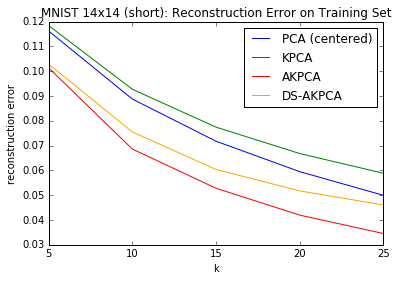
\includegraphics[scale=0.5]{figures/mnist_14_short_recon_training}
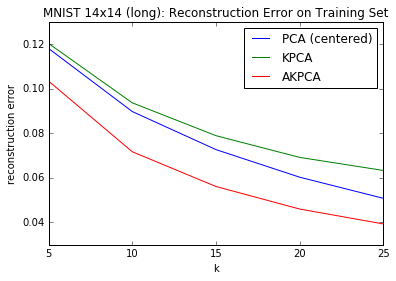
\includegraphics[scale=0.5]{figures/mnist_14_long_recon_training}
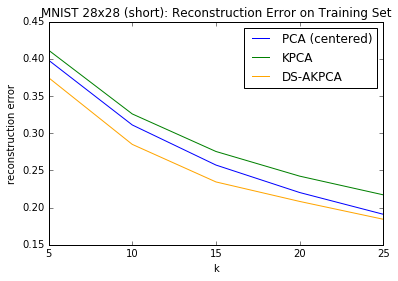
\includegraphics[scale=0.5]{figures/mnist_28_short_recon_training}
\caption{Average reconstruction error on the training set plotted as a function of number of components.  Top left: 14x14, short training set.  Top right: 14x14, long training set. Bottom: 28x28, short training set.}
\label{recon-err-training}
\end{center}
\end{figure}

Across all $k$, PCA with centering attained a lower reconstruction error than PCA without centering, so we do not report the performance of latter at all.

That DS-AKPCA did not perform as well as AKPCA suggests that the ``data-span'' assumption is incorrect: at the optimal solution, the rows of $\mathbf{A}$ and $\mathbf{B}$ do not lie within the span of the data points in feature space.


\subsubsection{Reconstuction Error on Held-Out Set}

The relative performance of all four algorithms on the training set remained the same on the held-out set, implying that none of the algorithms overfit too much.

\begin{figure}[h]
\begin{center}
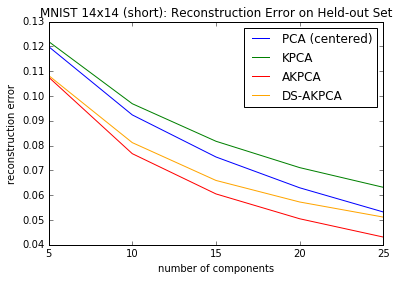
\includegraphics[scale=0.5]{figures/mnist_14_short_recon_testing}
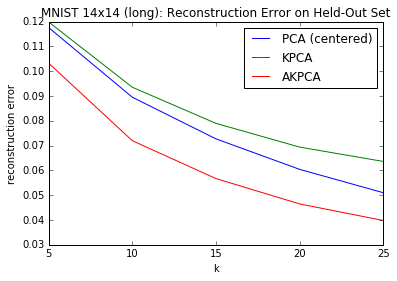
\includegraphics[scale=0.5]{figures/mnist_14_long_recon_testing}
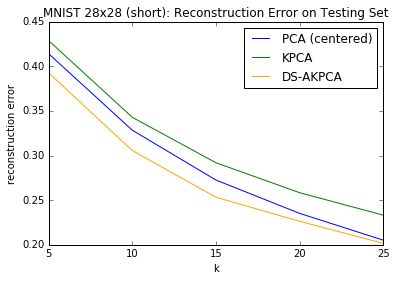
\includegraphics[scale=0.5]{figures/mnist_28_short_recon_testing}
\caption{Average reconstruction error on the held-out set, plotted as a function of number of components.  Top left: 14x14, short training set.  Top right: 14x14, long training set.  Bottom: 28x28, short training set.}
\end{center}
\end{figure}

Figure \ref{training-vs-test} compares reconstruction error on the training set and the held-out set for each algorithm.
The difference between the training and held-out reconstruction errors is a measure of how much the algorithm overfit to the training set.
As expected, overfitting is much greater with a short training set (left) than with a long training set (right).
In the small training set regime, AKPCA appears to overfit a bit more than the other three algorithms.

\begin{figure}[!ht]
\begin{center}
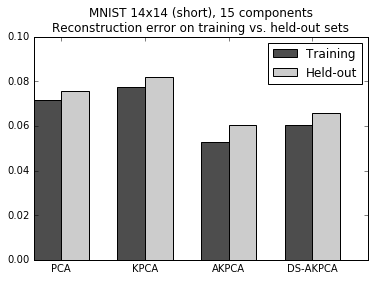
\includegraphics[scale=0.5]{figures/mnist_14_short_training_testing}
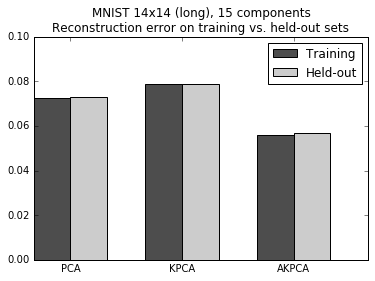
\includegraphics[scale=0.5]{figures/mnist_14_long_training_testing}
\caption{Average reconstruction error on the training vs. held-out set.  Left: short training set (300 examples per class).  Right: long training set (3,500 examples per class).}
\label{training-vs-test}
\end{center}
\end{figure}

Figure \ref{short-vs-long} illustrates the effect of training set size on generalization.
Across all algorithms, the larger the training set, the lower the reconstruction error on held-out data.

\begin{figure}[h]
\center
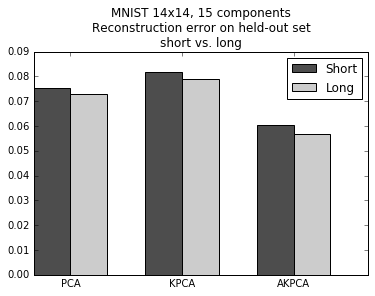
\includegraphics[scale=0.5]{figures/mnist_14_testing_short_long}
\caption{Comparing reconstruction error on held-out data for a model trained on a ``short'' training set (300 examples per class) vs. a ``long'' training set (1750 examples per class).  Across all algorithms, the model trained on a longer dataset exhibited lower (better) reconstruction error on held-out data.}
\label{short-vs-long}
\end{figure}

\subsubsection{Denoising: Gaussian Noise}

In the first denoising experiment, we pick an example $\mathbf{x}$ from the held-out set, add Gaussian noise $\boldsymbol{\epsilon} \sim \mathcal{N}(0, \sigma^2 \mathbf{I})$, and try to denoise $\mathbf{x} + \boldsymbol{\epsilon}$ by encoding with $f$ and then decoding with $g$.
We then measure the difference between the denoised version and the original example:
$$ \text{denoising error} = \frac{1}{n} \sum_{i = 1}^n \| g(f(\mathbf{x}_i + \boldsymbol{\epsilon}_i)) - \mathbf{x}_i  \|^2_2 \quad \text{where } \{ \mathbf{x}_i \}_{i=1}^n \text{ are the held-out data}$$

Figure \ref{gaussian-noise} shows several MNIST digits corrupted with increasing levels of Gaussian noise.

\begin{figure}[h]
\begin{center}

\includegraphics[scale=0.6]{{figures/digit_6700_noise_sd_0}}
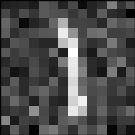
\includegraphics[scale=0.6]{{figures/digit_6700_noise_sd_2}}

\includegraphics[scale=0.6]{{figures/digit_6700_noise_sd_4}}
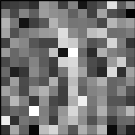
\includegraphics[scale=0.6]{{figures/digit_6700_noise_sd_6}}


\includegraphics[scale=0.6]{{figures/digit_13400_noise_sd_0}}

\includegraphics[scale=0.6]{{figures/digit_13400_noise_sd_2}}
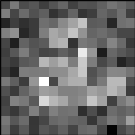
\includegraphics[scale=0.6]{{figures/digit_13400_noise_sd_4}}
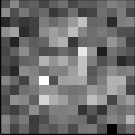
\includegraphics[scale=0.6]{{figures/digit_13400_noise_sd_6}}


\includegraphics[scale=0.6]{{figures/digit_20100_noise_sd_0}}

\includegraphics[scale=0.6]{{figures/digit_20100_noise_sd_2}}

\includegraphics[scale=0.6]{{figures/digit_20100_noise_sd_4}}

\includegraphics[scale=0.6]{{figures/digit_20100_noise_sd_6}}
\caption{Three MNIST digits corrupted by increasing levels of Gaussian noise.  From left to right, the standard devaiation of the noise is: $\{0, 0.02, 0.04, 0.06\}$. }
\label{gaussian-noise}
\end{center}
\end{figure}

The performance of all four algorithms on this denoising task is plotted in figure \ref{gaussian-denoising}.

Figure \ref{gaussian-denoising} shows the performance of all four algorithms at denoising MNIST digits corrupted by Gaussian noise.
The results were consistent across all three datasets, and across a model order of both 10 (top) and 20 (bottom).
Our algorithm AKPCA always performed the best at denoising so long as the standard deviation of the noise was small to moderately large.
As is clear from figure \ref{gaussian-noise}, a noise level of $\sigma = 0.04$ (third column from the left) is still a considerable amount of noise.

Additionally, the data-span variant of AKPCA outperformed PCA and KPCA in the high noise regime (though it did not perform as well as the standard AKPCA).

For Gaussian noise with $\sigma > 0.04$, kernel PCA generally gave the best denoising results.
\begin{figure}[h]
\begin{center}
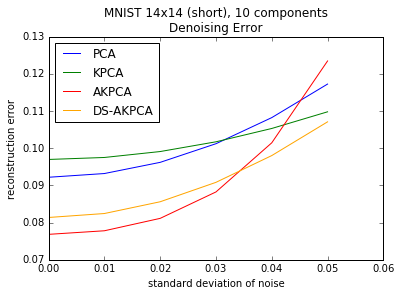
\includegraphics[scale=0.5]{figures/mnist_14_short_denoise_k10}
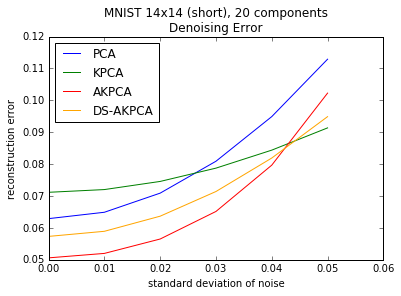
\includegraphics[scale=0.5]{figures/mnist_14_short_denoise_k20}

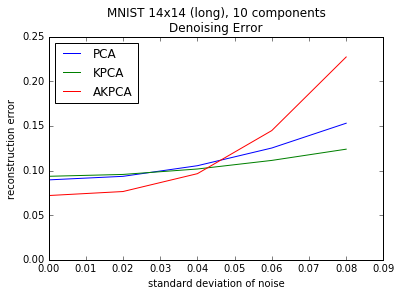
\includegraphics[scale=0.5]{figures/mnist_14_long_denoise_k10}
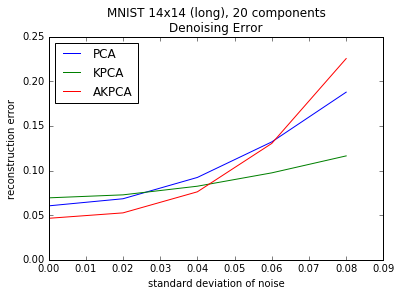
\includegraphics[scale=0.5]{figures/mnist_14_long_denoise_k20}

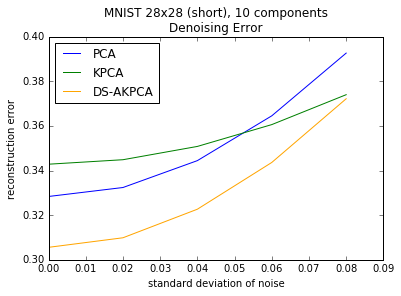
\includegraphics[scale=0.5]{figures/mnist_28_short_denoise_k10}
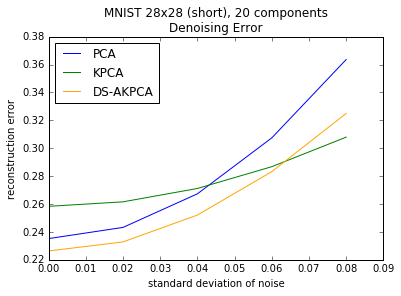
\includegraphics[scale=0.5]{figures/mnist_28_short_denoise_k20}
\caption{Denoising error of all four algorithms in denoising MNIST digits that have been corrupted by Gaussian noise, with 10 (left) and 20 (right) components in the model.}
\label{gaussian-denoising}
\end{center}
\end{figure}


\subsubsection{Denoising: Speckle Noise}

In the second denoising experiment, we pick a sample $\mathbf{x}$ from the held-out set, corrupt it with ``speckle'' noise \cite{mika1999} by independently setting each pixel to $0$ with probability $p$, and try to denoise the corrupted digit by encoding and then decoding.

Figure \ref{speckle-noise} shows three MNIST digits corrupted by increasing levels of ``speckle'' noise.

\begin{figure}[h]
\begin{center}
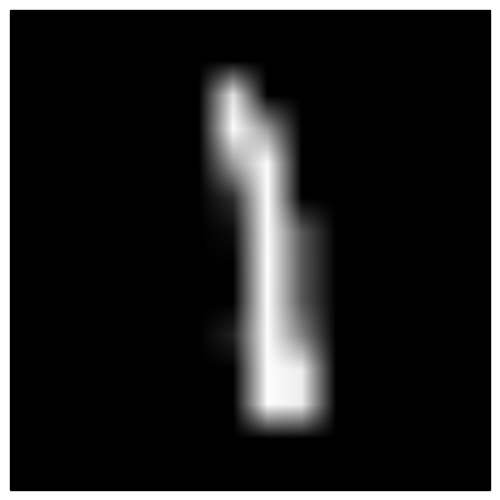
\includegraphics[scale=0.23]{{figures/digit_6700_prob_zero_0}}

\includegraphics[scale=0.23]{{figures/digit_6700_prob_zero_2}}

\includegraphics[scale=0.23]{{figures/digit_6700_prob_zero_3}}

\includegraphics[scale=0.23]{{figures/digit_6700_prob_zero_4}}

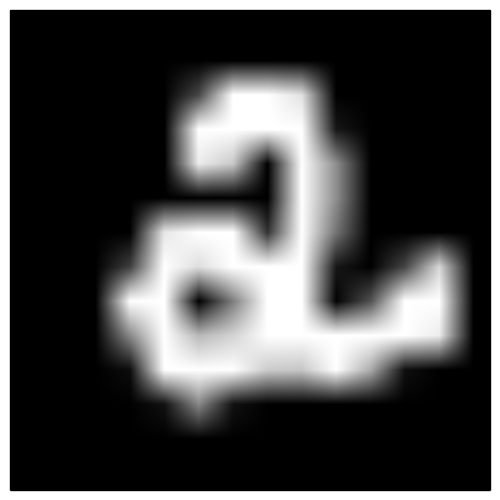
\includegraphics[scale=0.23]{{figures/digit_13400_prob_zero_0}}

\includegraphics[scale=0.23]{{figures/digit_13400_prob_zero_2}}
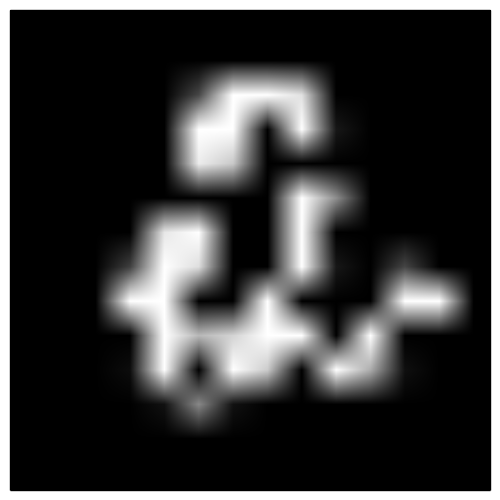
\includegraphics[scale=0.23]{{figures/digit_13400_prob_zero_3}}
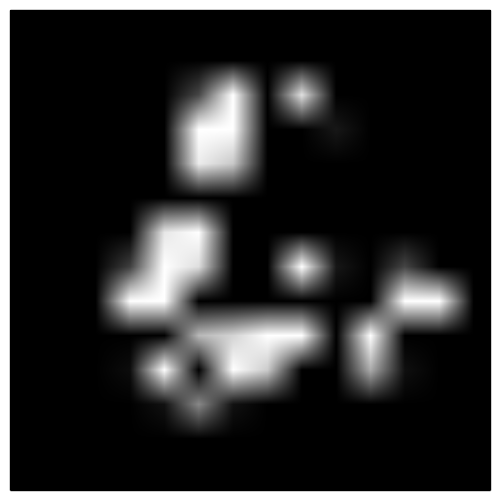
\includegraphics[scale=0.23]{{figures/digit_13400_prob_zero_4}}

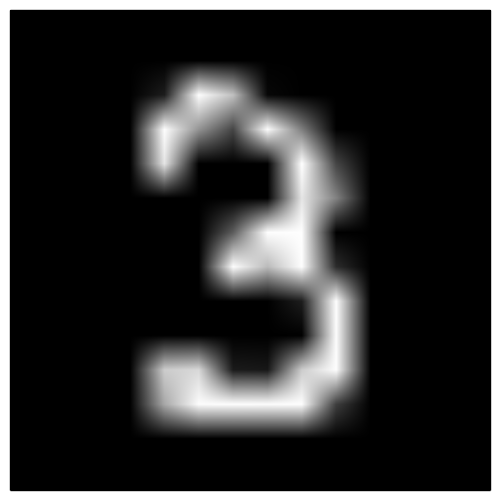
\includegraphics[scale=0.23]{{figures/digit_20100_prob_zero_0}}
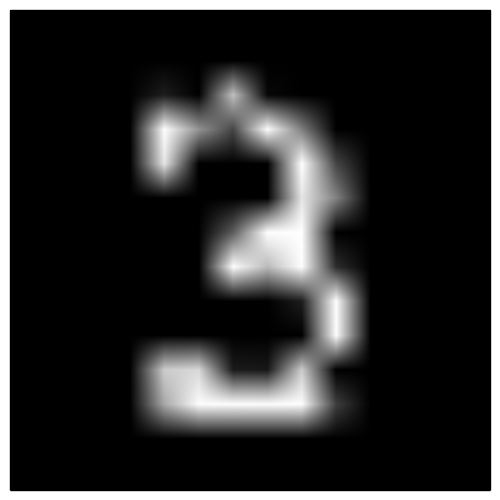
\includegraphics[scale=0.23]{{figures/digit_20100_prob_zero_2}}
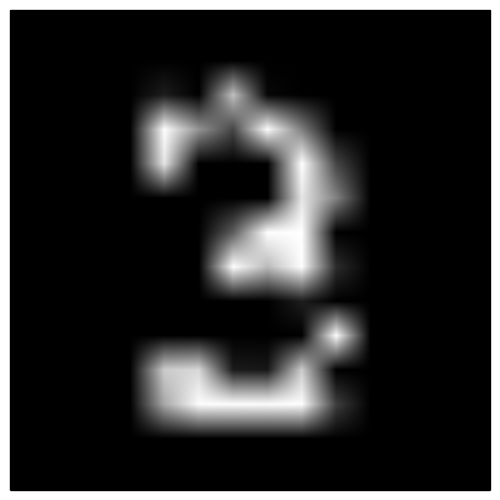
\includegraphics[scale=0.23]{{figures/digit_20100_prob_zero_3}}
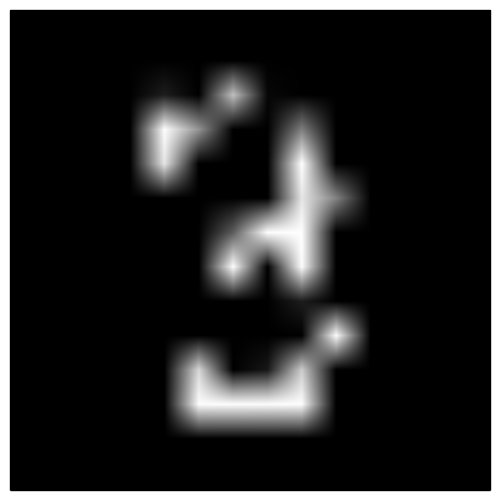
\includegraphics[scale=0.23]{{figures/digit_20100_prob_zero_4}}
\caption{Three MNIST digits corrupted by increasing levels of speckle noise.  From left to right: $p$, the probability that a pixel is set to zero, is varied in $\{0, 0.2, 0.3, 0.4\}$.}
\label{speckle-noise}
\end{center}
\end{figure}

Figure \ref{speckle-denoising} shows the denoising error of all four algorithms at denoising digits corrupted by speckle noise, for models of 10 (left) and 20 (right) components.
For the 14x14 datasets, our algorithms, AKPCA and DS-AKPCA, outperform PCA and kernel PCA under all conditions studied.
For the 28x28 dataset, DS-AKPCA outperforms PCA and KPCA so long as the noise is low to moderate.

\clearpage

\begin{figure}[!h]
\begin{center}
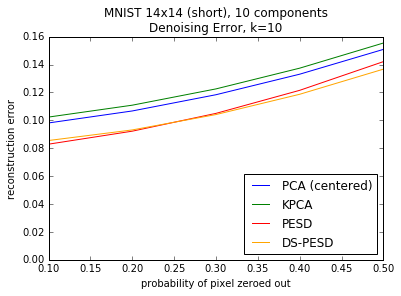
\includegraphics[scale=0.5]{figures/mnist_14_short_speckle_k10}
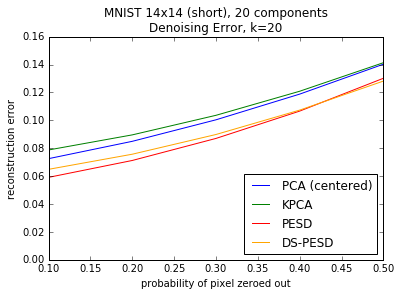
\includegraphics[scale=0.5]{figures/mnist_14_short_speckle_k20}

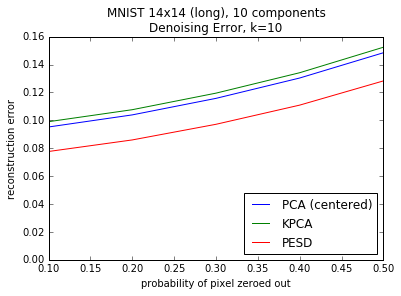
\includegraphics[scale=0.5]{figures/mnist_14_long_speckle_k10}
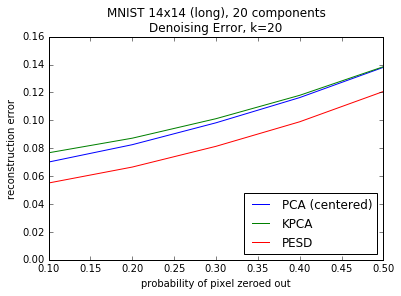
\includegraphics[scale=0.5]{figures/mnist_14_long_speckle_k20}

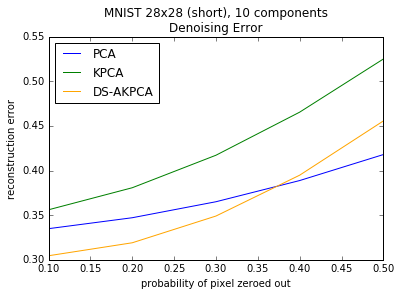
\includegraphics[scale=0.5]{figures/mnist_28_short_speckle_k10}
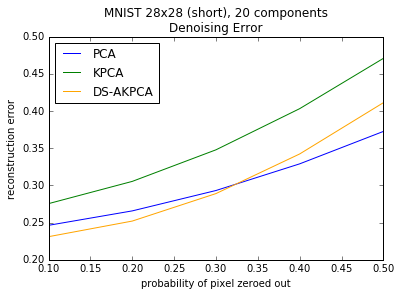
\includegraphics[scale=0.5]{figures/mnist_28_short_speckle_k20}
\caption{Denoising error of all four algorithms in denoising MNIST digits that have been corrupted with speckle noise, as a function of $p$, the probability that a pixel is set to zero.  Plots shown for models of 10 (left) and 20 (right) components.}
\label{speckle-denoising}
\end{center}
\end{figure}

\subsubsection{Classification}

The goal of the classification experiment was to evaluate whether the encoding function learned by each algorithm serves well as a preprocessing step for the 10-way classification task of discriminating digits.
For each of PCA, KPCA, AKPCA, and DS-AKPCA, we learned an encoder $f$ on the training set and then used $f$ to encode the held-out set.
We trained a linear classifier on a portion of the encoded held-out set and measured its accuracy on the remainder, using cross-validation to average the classification accuracy over several training / testing splits.

For the linear classifier, we used logistic regression with a ``multinomial'' or ``softmax'' loss.
The probability that a data point $\mathbf{x} \in \reals^k$ belongs to class $c$ is modeled as:
$$ p(y = c | \mathbf{x}) = \frac{\mathbf{w}_c^T \mathbf{x}}{\sum_{j=1}^C \mathbf{w}_j^T \mathbf{x}}$$
and the parameters $\mathbf{w}_1 \hdots \mathbf{w}_C \subseteq \reals^k$ are learned by maximizing the likelihood of the training data labels. 

We tried training the classifier on both a small training set (18 examples per class) and a large training set (1750 examples per class).

Figure \ref{classification-accuracy} plots cross-validated classification accuracy as a function of number of components, for short (left) and long (right) dimensionality reduction training set sizes, and small (top) and large (bottom) classification training set sizes.
The only regime where AKPCA outperformed its competitors across all model orders was when both the dimensionality reduction training set and the classification training set were small (upper left corner).
In all other settings, KPCA and occasionally PCA outperformed AKPCA for large enough model order ($k \ge 20$).

\begin{figure}[h]
\begin{center}
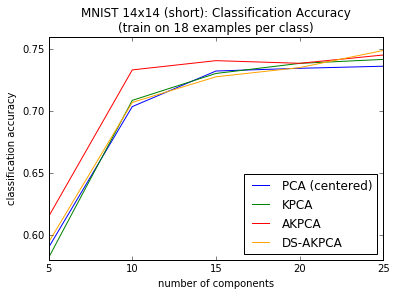
\includegraphics[scale=0.5]{figures/mnist_14_short_classify_18}
\includegraphics[scale=0.5]{figures/mnist_14_short_classify_1750}

\includegraphics[scale=0.5]{figures/mnist_14_long_classify_18}
\includegraphics[scale=0.5]{figures/mnist_14_long_classify_1750}

\includegraphics[scale=0.5]{figures/mnist_28_short_classify_18}
\includegraphics[scale=0.5]{figures/mnist_28_short_classify_1750}
\caption{Cross-validated classification accuracy as a function of number of components, for small (left) and large (right) classification training set sizes.}
\end{center}
\label{classification-accuracy}
\end{figure}

\clearpage

\section{Conclusion}

The ``autoencoder principle'' is that a dimensionality reduction algorithm learns informative structure if it learns an \textit{encoder} that compresses data into a low-dimensional encoding, and a \textit{decoder} that reconstructs the original data from the encodings.
Principal component analysis can be derived from the autoencoder principle, yet it is limited by the underlying assumption that the data lie close to a linear subspace.
On the other hand, kernel PCA can discover nonlinear structure, yet does not have an autoencoder interpretation.
In this technical report, we presented autoencoding kernel PCA (AKPCA), an algorithm derived from the autoencoder principle which can learn non-linear structure.
AKPCA learns to compress the degree-2 polynomial expansion of a data point into a low-dimensional encoding, and to reconstruct the original data point from there.
We also presented a ``data-span'' variant of AKPCA which scales better to datasets with high dimensionality, provided that the number of data points is small.

We showed that AKPCA and DS-AKPCA outperform PCA and kernel PCA with a degree-2 polynomial kernel at a denoising task on the MNIST dataset.
Unfortunately, results on a classification task were mixed --- our two algorithms generally matched PCA and KPCA in classification accuracy, but failed to consistently outperform them.
Likewise, our algorithms did not perform well at compressing the CIFAR-10 or LFW datasets.

A final drawback to the two algorithms we propose is that they are computationally expensive: whereas PCA takes seconds on the datasets we consider, and kernel PCA takes minutes at most, our algorithms require a runtime on the scale of hours, since they perform stochastic gradient descent on a non-convex objective.

\begin{thebibliography}{9}

\bibitem{kwok2003}
James Kwok and Ivor Tsang.
``The Pre-Image Problem in Kernel Methods.''
\textit{International Conference on Machine Learning.}
2003.

\bibitem{johnson2013}
Rie Johnson and Tong Zhang.
``Accelerating Stochastic Gradient Descent using Predictive Variance Reduction.''
\textit{Advances in Neural Information Processing Systems.}
2013.

\bibitem{mika1999}
Sebastian Mika, Bernhard Scholkopf, Alex Smola, Klaus-Robert Muller, Matthias Scholz, and Gunnar Ratsch.
``Kernel PCA and De-Noising in Feature Spaces.''
\textit{Advances in Neural Information Processing Systems.}
1999.

\bibitem{scholkopf2002}
Bernhard Scholkopf and  Alexander Smola.
\textit{Learning with Kernels}.
2002.

\bibitem{scholkopf1997}
Bernhard Scholkopf, Alexander Smola, and Klaus-Robert Muller.
``Kernel Principal Component Analysis.''
\textit{International Conference on Artificial Neural Networks.}
1997.

\bibitem{williams2001}
Christopher Williams and Matthias Seeger.
``Using the Nystrom Method to Speed Up Kernel Machines.''
\textit{Advances in Neural Information Processing Systems}.
2001.

\end{thebibliography}



\end{document}